%!TEX root = ../../thesis.tex
	Acknowledgment: Florian, Akitoshi
	\section{Introduction}
		As seen in Chapter \ref{section:real_complexity} many important operators 
		on real functions have been shown to be computationally hard.
		On the other hand, numerical scientists can quickly compute maximums or anti-derivatives of functions.
		To analyze this mismatch one should ask the following questions
		\begin{enumerate}
			\item What subset of real functions is usually considered in numerical analysis?
			\item Are there implicit assumptions made about the functions, that allow faster computations? 
		\end{enumerate}
		One class of functions that has been considered in computable analysis is the analytic functions.
		Although not at all sufficient as the class of functions considered interesting for numerical analysis, 
		many computations become tractable when one restricts the attention to analytic functions.
		\begin{definition}
			For $z \in \CC$ and $r \in \RR, r > 0$, let $B(z,r) := \{ x \in \CC \,\, | x - z | < r\}$. \\
			A function $f: D \to \CC$ with $D \subseteq CC$ is called \textbf{analytic} if for every $x_0 \in D$ 
			the function given by the Taylor-series around $x_0$ converges to $f(x)$ for every $x$ in a neighborhood of 
			$x_0$. \\
			That is, for every $x_0 \in D$ there is an $\varepsilon > 0$, such that for all $x \in B(x_0, \varepsilon)$ and there is a series
			$$ T(x) := \sum_{n=0}^{\infty} a_n(x-x_0)^n$$
			such that $T(x) \rightarrow f(x)$.

		\end{definition}
		The above definition can be easily generalized to higher dimension. \\
		If $f$ is analytic then all its derivatives $f^{(n)}(x)$ exist and it holds
		$$ a_n = \frac{f^{(n)}(x_0)}{n!}. $$    

		The set of functions analytic on $D$ will be denoted by $C^\infty(D)$. \\		
		For the sake of simplicity, it will w.l.o.g. be assumed that $x_0 = 0$ if not stated otherwise.
		
		Below are some properties of analytic functions

		\begin{enumerate}
			\item For $f,g \in C^\infty(D)$ the sum  $f+g$ and the product $fg$ are analytic functions.
			\item If $f, g$ are analytic and $im(f) \subseteq dom(g)$ then their composition $f \circ g$ is analytic.
			\item The roots of an analytic function that is not identical to $0$ are isolated points.
			\item The derivative and anti-derivative of an analytic function are analytic.
			\item If the domain is connected, an analytic function is uniquely defined by a single Taylor series around one point in its domain.
		\end{enumerate}

		Analytic functions have been thoroughly investigated in real number complexity theory.
		For many problems that are hard in the general case, it could be shown that polynomial time algorithms exist when restricting the input to
		analytic functions.

		\begin{theorem}[Pour-El, Richards, Ko, Friedman]\label{theorem:computable equiv series computable} 
			The following are equivalent
			\begin{enumerate}
				\item $f$ is computable 
				\item The series $(a_n)_{n \in \NN}$ is computable. 
 			\end{enumerate}
		\end{theorem}
		\begin{theorem}[M\"uller]\label{theorem:computable equiv series computable polytime}
			The equivalence in Theorem \ref{theorem:computable equiv series computable} also holds, when the word computable is replaced by polynomial time computable.
		\end{theorem}
		
		Since differentiation and anti-differentiation on analytic functions are only simple manipulations on the series, 
		a direct consequence of Theorem \ref{theorem:computable equiv series computable polytime} is the following
		\begin{corollary}
			If $f \in C^\omega(D)$ is polynomial time computable the following functions are also polynomial time computable:
			\begin{enumerate}
				\item $i: D \to \RR$, $i(x) = \int_0^x f(t) dt$
				\item $d: D \to \RR$, $d(x) = f'(x)$ 
			\end{enumerate}
		\end{corollary}
		
		The above theorems show that computing with analytic functions is in some sense much easier than the general case.

		However, those theorems are non-uniform in the following sense:

		The theorems only say that, that $f$ being polynomial time computable implies the existence of a polynomial time computable sequence
		and the existence of such a sequence implies that there exists some algorithm computing $f$ in polynomial time. \\
		In no way, however, do they say, how to compute the sequence from a given representation of the function and vice versa.

		In fact the following theorems show, that this is not a problem of those theorems, but it's inherently impossible to do so.
		\begin{theorem}[M\"uller \cite{Mue}]
			Let $f$ given as in ... then the operator $f \to (a_n)_{n \in \NN}$ computing the Taylor series around $0$ (or any other point) is not computable.
		\end{theorem} 
		\begin{theorem}[M\"uller \cite{Mue}]\label{theorem: evaluation not uniformly computable from powerseries}
			Let $(a_n)_{n \in \NN}$ be the series expansion around $0$ for some $f \in C^\omega(D)$.\\
			The evaluation operator $((a_n)_{n \in \NN}, x) \to f(x)$ that, given a series and a point, computes the value of the corresponding function at that point, is not computable.
		\end{theorem} 

		The reason for Theorem \ref{theorem: evaluation not uniformly computable from powerseries} is, that any algorithm can only read a finite number of 
		coefficients from the series. But from the power series alone, it is impossible to know how many coefficients are needed to make
		a good enough approximation. 

		The goal of the case study is to write a general data type for analytic functions. 
		Due to the above any such data type will need more information than only the series of Taylor coefficients. \\
		The next section will deal with the question, what additional information is needed to get uniform versions of the above theorems.

	\section{Representation of Analytic Functions}
	 As seen in the previous section, the information given by the series expansion is not enough to represent an analytic function.
	 However, by enriching the information by some finite discrete parameters, the translation between Taylor-series and function representation can be made uniform.
	 
	 Two possible representations for analytic functions on the closed unit disc are as follows
	 \begin{definition}\label{def:series_name_ball}
	 	A \textbf{series-name} $\rho_s$ of $f \in C^\omega(\overline{B_1(0)})$ is a triple $((a_n)_{n \in \NN}, k, A)$ where 
	 	\begin{enumerate}
	 		\item $(a_n)_{n \in \NN}$ is the series expansion of $f$ around $0$
	 		\item $\sqrt[k]{2} \leq R$ 
	 		\item $|a_j|r^j \leq A$ for all $j \in \NN$
	 	\end{enumerate}
	 	and $R = (\limsup |a_j|^{\frac{1}{j}})^{-1}$ denotes the radius of convergence of the series.
	 \end{definition}
	 The two additional parameters are useful, because they can be used to make a tail estimate 
	 \begin{equation}\label{eqn:tail_estimate}
	  \left | \sum_{n \geq N} a_nx^n \right | \leq A \frac{(|z|/r)^N}{1-|z|/r}
	 \end{equation}
	 A name as in Definition \ref{def:series_name_ball} can be found by choosing any appropriate $k$ (note that the radius of convergence is always bigger than $1$) and choosing $A$ as an upper bound of $f$ extended to $\overline{B_{\sqrt[k]{2}}(0)}$. 
	 \begin{definition}\label{def: function name ball}
	 	A \textbf{function-name} $\rho_f$ of $f \in C^\omega(\overline{B_1(0)})$ is a triple $(f, l, B)$ such that
		B is an upper bound of $f$ on $\overline{B_{\sqrt[l]{2}}(0)}$.
	 \end{definition}
	 \begin{theorem}\cite{Kaw}\label{thm:representation_conversion}
	 	The mapping between $\rho_s$-name and $\rho_f$-names is computable in time polynomial in 
	 	$n+k+\log(A)$ and the inverse mapping is computable in time polynomial in $n+l+\log(B)$ 
	 \end{theorem}
	 A full proof of Theorem \ref{thm:representation_conversion} can be found in \cite{Kaw}. 
	 Some of the details that are important for the implementation are given below.
	 \begin{proof}[Sketch]
	 	To compute a function name from a series name it only has to be shown that the series name can be used to evaluate the function and that the two parameters can be computed.
		


	 	To compute a series name from a function name, one has to compute the coefficients of the series expansion from a function name, i.e. from the function and the parameters $l$ and $B$.
	 	In \cite{Mue} M\"uller describes an algorithm for this task.
	 	To approximate the coefficient $a_k$ with precision at least $2^{-n}$ $f$ is approximated by the Lagrangian interpolation
	 	polynomial
	 	\begin{equation}\label{eqn:interpolation_polynomial}
	 		P_m(x)  :=  \sum_{i=0}^{2m} f(x_i) \cdot L_{m,i}(x) 
	 	\end{equation}
	 	where
	 	\begin{eqnarray*}
	 		x_i & = & (i-m) \cdot h , h \in \RR, h > 0 \\
	 		L_{m,i}(x) & = & \prod_{i \neq j} \frac{x-x_j}{x_i-x_j} 
	 	\end{eqnarray*}
	 	Differentiating Equation \ref{eqn:interpolation_polynomial} $k$ times yields
	 	\begin{equation}\label{eqn:interpolation_polynomial_diff}
	 		P_m^k(0)  :=  \sum_{i=0}^{2m} f(x_i) \cdot L_{m,i}^{(k)}(x) 
	 	\end{equation}
	 	Let $\sigma = \lceil \log_2 B \rceil + 1$

	 	It can then be shown that if $f$ is evaluated on $2k+1$ points from the 
	 	real interval $\{x \in \R \,|\, |x| \leq \frac{1}{2}\}$ with precision $2n+15k+\sigma+6$ 
	 	then $a_k$ can be approximated by the above procedure with error less than $2^{-n}$ in 
	 	$O((k+1)\cdot \M(n+k+\sigma) + k^2 \M (k \log k)$

	 \end{proof}
	 Note that the above translation becomes fully polynomial time when in the representations $k$ resp. $l$ are required to be encoded in unary, while $A$ resp. $B$ are given in binary.
	 Thus, from now on the term polynomial time computable will be used when referring to running time bounds as in Theorem \ref{thm:representation_conversion}.
	 \begin{theorem}\label{thm:polytime_on_ball}
	 	The following is polynomial time computable when given $\rho_s$ or $\rho_f$ names for the input functions.
	 	\begin{enumerate}
	 		\item Evaluation $(f,z) \to f(z)$
	 		\item Addition $(f_1, f_2) \to f_1 + f_2$
	 		\item Multiplication $(f_1, f_2) \to f_1 \cdot f_2$
	 		\item $d$-fold Differentiation $(f,d) \to f^{(d)}$ where $d$ is given as unary
	 		\item $d$-fold Anti-differentiation $(f,d) \to \int \dots \int f$ where $d$ is given in unary
	 		\item Parametric maximization
	 	\end{enumerate}
	 	\begin{proof}(Sketch)
	 		Evaluation follows from \ref{thm:representation_conversion}. \\
	 		Except for parametric maximization the manipulations that have to be done on the Taylor series are straight forward (e.g. for addition, just add the coefficients).
	 		It remains to show how to compute the new parameters $A'$ and $k'$. 
	 	\end{proof}
	 \end{theorem}

	The above can be extended to a data type for analytic functions on arbitrary ball-shaped domains.\\
	But of course, most domains are not ball-shaped and one would also like to represent such domains.
	
	One possible way to represent such functions, is to cover the domain with balls and use the representation from Definition \ref{def:series_name_ball} on each ball.
	As an example, consider functions analytic on the real line $[-1,1]$ (this implies being analytic on a rectangle around the line $[-1,1]$ in the complex plane).
	

	 \begin{figure}
	 	\centering
	 	\begin{subfigure}{.45\textwidth}
	 		\centering
			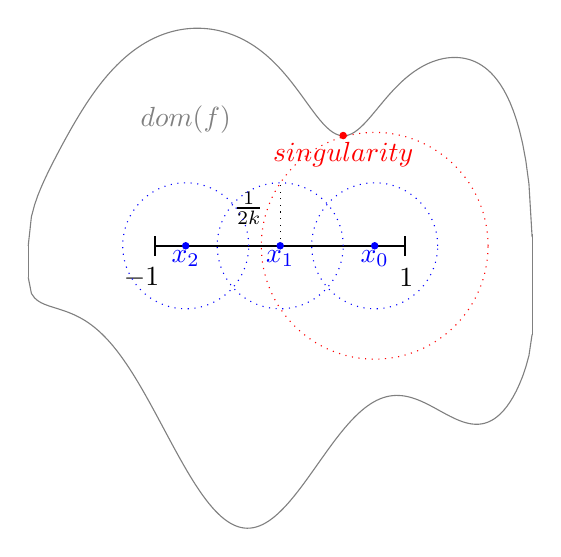
\begin{tikzpicture}[scale=0.8]
			    \node  at (-0.2,-0.5) {$-1$};
			    \node  at (4.0,-0.5) {$1$};
			    \draw [thick,|-|] (0,0) -- (4,0);
			    \node  at (1.5,.6) {$\frac 1{2k}$};
			    \draw  [dotted] (2.0,0) -- (2.0,1);
			    \draw [domain = 0:8,color=gray] plot[samples=160] (\x-2, {sqrt(16-(\x-4)^2)*(1-1/(\x^2+1) + sin(\x) + (\x/7)^5-\x/6 +1.5- 1/((\x-5)^2+1))/2});
			    \draw [domain = 0:8,color=gray] plot[samples=160] (\x-2, {1/(\x^2+1)/2 + sin(80*\x) + (\x/7)^5-\x/6 -1-sqrt(16-(\x-4)^2)/2});
			    \draw [color=gray] (-2,0) -- (-2,-.5);
			    \draw [color=gray] (6,.19) -- (6,-1.42);
			    \node [color=gray] at (.5,2) {$dom(f)$};
			    \draw [fill=blue,radius =.05,color=blue] (3.5,0) circle;
			    \node [color=blue] at (3.5,-.2) {$x_0$};
			    \draw [fill=blue,radius =.05,color=blue] (2.0,0) circle;
			    \node [color=blue] at (2.0,-.2) {$x_1$};
			    \draw [radius = 1,color=blue, dotted] (2.0,0) circle; 
			    \draw [fill=blue,radius =.05,color=blue] (0.5,0) circle;
			    \node [color=blue] at (0.5,-.2) {$x_2$}; 
			    \draw [radius = 1,color=blue, dotted] (0.5,0) circle;
			    \draw [radius = 1,color=blue, dotted] (3.5,0) circle;
			    \draw [radius = 1.8, color = red, dotted] (3.5,0) circle; 
			    \draw [fill=red,radius = .05,color = red] (3,1.75) circle;
			    \node [color=red] at (3,1.45) {$singularity$};
			\end{tikzpicture}
			\caption{For a series name the domain is covered with equally sized balls. 
			For each ball a Taylor series around the center of the ball is given and the properties of Definition \ref{def:series_name_ball} hold.}\label{fig: analytic function representation series name}
		\end{subfigure}
		\centering
	 	\begin{subfigure}{.45\textwidth}
			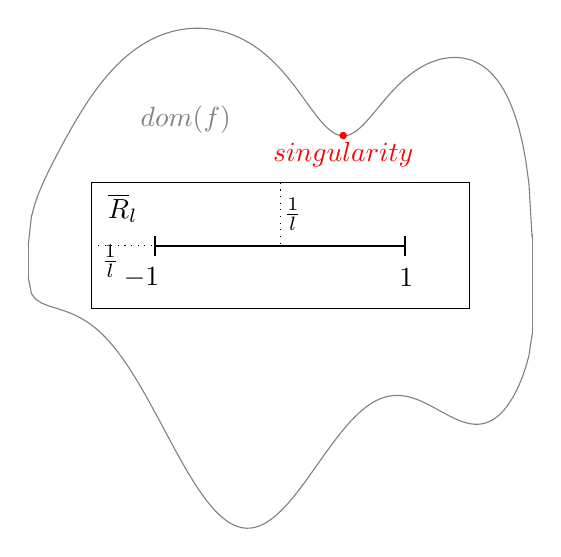
\begin{tikzpicture}[scale=0.8]
			    \draw (-1,1) rectangle (5,-1);
			    \node  at (-0.2,-0.5) {$-1$};
			    \node  at (4.0,-0.5) {$1$};
			    \draw [thick,|-|] (0,0) -- (4,0);
			    \node  at (-.7,-.25) {$\frac 1l$};
			    \draw  [dotted] (-1,0) -- (0,0);
			    \node  at (2.2,.5) {$\frac 1l$};
			    \draw  [dotted] (2,1) -- (2,0);
			    \node  at (-.5,0.6) {$\overline R_l$};
			    \draw [domain = 0:8,color=gray] plot[samples=160] (\x-2, {sqrt(16-(\x-4)^2)*(1-1/(\x^2+1) + sin(\x) + (\x/7)^5-\x/6 +1.5- 1/((\x-5)^2+1))/2});
			    \draw [domain = 0:8,color=gray] plot[samples=160] (\x-2, {1/(\x^2+1)/2 + sin(80*\x) + (\x/7)^5-\x/6 -1-sqrt(16-(\x-4)^2)/2});
			    \draw [color=gray] (-2,0) -- (-2,-.5);
			    \draw [color=gray] (6,.19) -- (6,-1.42);
			    \node [color=gray] at (.5,2) {$dom(f)$};
			    \draw [fill=red,radius = .05,color = red] (3,1.75) circle;
			    \node [color=red] at (3,1.45) {$singularity$};
			    %\draw [radius = 1, color = blue, dotted] (2.5,0) circle;
			    %\draw [fill=blue, radius = .05, color = blue] (2.5,0) circle;
			    %\node [color=blue] at (2.5,-.2) {$x_1$};
			\end{tikzpicture}
			\caption{A function name encodes a closed rectangle around $[-1,1]$ where the function is analytic and an upper bound for the function on that rectangle.}\label{fig: analytic function representation function name}
		\end{subfigure}
		\caption{Representations for functions analytic on the real line $[-1,1]$}\label{fig: analytic function representations}
	 \end{figure}
	\begin{definition}\label{def:series_name_rect}
		Let $f \in C^\omega([-1,1])$.
		A \textbf{series-name} for $f$ is a 5-tuple $(M, (x_m), (a_{n, j}), k, A)$ where $M \in \NN$
		$1 \leq j \leq M$, $n \in \NN$, $x_m \in [-1,1]$ and it holds
		\begin{enumerate}
			\item $[-1,1] \subseteq \bigcup_{m=1}^M [x_m - \frac{i}{4k}, x_m + \frac{1}{4k}]$
			\item $(a_{n,i})_{n \in \NN}$ is the series expansion of $f$ around $x_i$
			\item $|a_{n,i}| \leq Ak^n$ for all $n \in N$, $1 \leq i \leq M$
		\end{enumerate}
	\end{definition}
	To simplify the definition the parameters $k$ and $A$ were chosen global, i.e. they hold for each of the series.
	That means, the domain is covered by equally sized balls. 
	Figure \ref{fig: analytic function representation series name} shows a series name with three series.
	
	The definition can be further simplified by requiring the series centers to be equidistantly distributed on $[-1,1]$ and thus
	making it unnecessary to store them in the representation.

	A function name as in Definition \ref{def: function name ball} can also be defined
	\begin{definition}
		Let $R_l := [-\frac{1}{l}, 1+\frac{1}{l}] \times [-\frac{1}{l}, \frac{1}{l}]$ the closed rectangle with distance $\frac{1}{l}$ around $[-1,1]$ .\\
		A \textbf{function-name} for a function $f \in C^\omega([-1,1])$ is a 3-tuple $(f|_{[-1,1]}, B, l)$ with $B, l \in \NN$ such that 
		\begin{enumerate}
			\item $f \in C^\omega(R_l)$
			\item $B$ is an upper bound for $f$ on $R_l$
		\end{enumerate}
		where $l$ is coded in unary and $B$ in binary.
	\end{definition}
	Figure \ref{fig: analytic function representation function name} visualizes the function name. 

	Again it can be shown that the two representations are polynomial time equivalent, and that the equivalent to
	Theorem \ref{thm:polytime_on_ball} holds.
	\section{Analytic Continuation}
		One problem with the representation in Definition \ref{def:series_name_rect} is that when thinking of this representation as an interface for a data type, it is very cumbersome for the user to provide all the information needed. 
		He would need to give an algorithm for as many Taylor series as needed to cover the interval.
		\begin{figure}
			\centering
			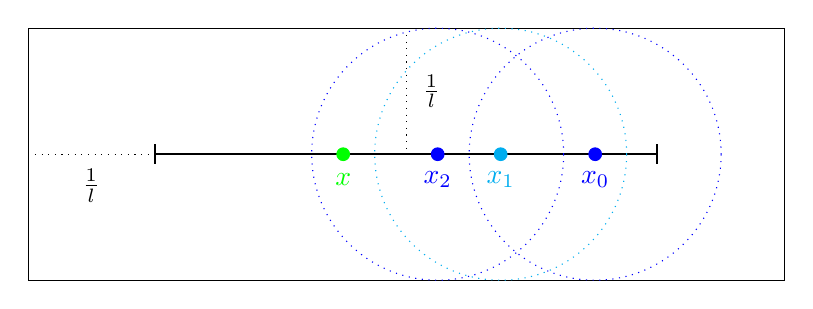
\begin{tikzpicture}[scale=1.6]
			    \draw (-1,1) rectangle (5,-1);
			    \draw [thick,|-|] (0,0) -- (4,0);
			    \node at (-.5,-.25) {$\frac 1l$};
			    \draw [dotted] (-1,0) -- (0,0);
			    \node at (2.2,.5) {$\frac 1l$};
			    \draw [dotted] (2,1) -- (2,0);
			    \draw [fill=blue,radius =.05,color=blue] (3.5,0) circle;
			    \node [color=blue] at (3.5,-.2) {$x_0$};
			    \draw [radius = 1,color=blue, dotted] (3.5,0) circle;
			    \draw [fill=green, radius = .05, color = green] (1.5,0) circle;
			    \node [color=green] at (1.5,-.2) {$x$};
			    \draw [fill=cyan, radius = .05, color = cyan] (2.75,0) circle;
			    \node [color=cyan] at (2.75,-.2) {$x_1$};
			    \draw [radius = 1,color=cyan, dotted] (2.75,0) circle;
			    \draw [fill=blue, radius = .05, color = blue] (2.25,0) circle;
			    \node [color=blue] at (2.25,-.2) {$x_2$};
			    \draw [radius = 1,color=blue, dotted] (2.25,0) circle;
			\end{tikzpicture}
			\caption{Evaluation by Analytic Continuation: 
					to evaluate the function at point $x$ given the series around $x_0$, first the series around 
					point $x_1$ is computed. This series is used to compute one more series around $x_2$ which then finally
					can be evaluated at $x$.}\label{fig: analytic continuation}
		\end{figure}
		As said before, there is no real gain of information by providing all those series.
		The analytic function is uniquely defined by the Taylor series around a single point.
		Thus, one would like to have something like the following representation
		\begin{definition}
			A \textbf{single series name} for $f \in C^\omega([-1,1])$ is a quadruple $(x_0, (a_n)_{n \in \NN}, k, A)$ such that
			\begin{enumerate}
				\item $(a_n)_{n \in \NN}$ is the series expansion of $x$ around $x_0$
				\item $A$ and $k$ are such that $| a_m | \leq Ak^m$ 
			\end{enumerate}
		\end{definition}
		A series name can be computed from a single series name by computing the series expansion on another point on the domain and then iterating this process until the series cover $[-1,1]$.

		Since the parameters $A$ and $k$ are such that they hold on the entire rectangle, 
		the new series will be valid on a ball with the same radius as the original series, effectively extending the domain.
		This process is called \textbf{analytic continuation},
		
		The series can be computed either by applying the algorithm from the proof of Theorem \ref{thm:representation_conversion} or by directly computing the derivatives at an other point using Theorem \ref{thm:polytime_on_ball}.
		Note however, that iterating this process will break the polynomial time computability, as will be shown in the next
		section.
	\section{Complexity Analysis}
		The previous section gave an overview of the representations and how they can be used to yield efficient 
		operations on analytic functions, where efficient means polynomial time computable.
		Since for practical applications polynomial time computability is too coarse a measure for efficiency, 
		in this section a more refined analysis on the algorithms is done, to establish time bounds in terms of $O$-notation.
		Most of this was already done in \cite{mypaper}.
		Of course, the overall running time will depend on the running time $T(a_m, n)$ that is needed to 
		compute the coefficient $a_m$ with error less than $2^{-m}$.
		\begin{theorem}
			Given a series name of $f \in C^\omega(D)$.
			To evaluate $f$ with error less than $2^{-n}$ 
			$$N = k(n+\lceil log_2(log_2 (e^2) kA \rceil)$$
			coefficients of the Taylor series are sufficient. \\
			This yields evaluation computable in time 
			$$ O(N\M(N)+N \cdot T(a_N, n+log_2(N)+1)) $$ 
		\end{theorem}

		\begin{theorem}
			Computing the $m$-th coefficient of the series for the $d$-fold derivative can be done
			$$ O(T(a_{m+d}, n+d\log_2(d+m)))+d\M(d \log_2 (d+m)+n)) $$
		\end{theorem}

		\begin{theorem}
			Given a series name of $f \in C^\omega(D)$, the number of coefficients of the series of the $d-fold$ derivative computed from $f$ as in Theorem \ref{thm:polytime_on_ball} needed to evaluate this derivative, is given by 
			$$N_d = k\left(n+\lceil log_2(log_2 (e^4) kA \rceil+\left \lceil d\left(\log_2(d)+\log_2(\log_2(e)k+1)-\frac{1}{k}\right)\right\rceil\right).$$
			Thus, evaluating the $d$-fold derivative of $f$ is possible in time bound by
			$$ O(N_d\M(N)+N_d \cdot T(a_{N_d+d}, n+d\log_2(d+N_d)))+d\M(d \log_2 (d+N_d)+n) $$ 
		\end{theorem}
		For computing the $m$-th coefficient of a Taylor series around some point the $m-th$ derivative 
		has to be divided by $m!$. This division reduces the needed precision leading to 
		$$N_{coeff}(m) = 2k\left( n+\lceil log_2(\log_2 (e^4) kA) + m \log_2(log_2(e)k+1)\rceil \right)$$
		as the number of coefficients that are needed to compute the $m-th$ coefficients of the Taylor series 
		around another point. 
		For stepwise analytic continuation it is necessary to iterate the process of differentiating.
		For example, using the single series name when one wants to evaluate the function at a point $x$
		that is not inside the ball of the given series, analytic continuation has to be applied until a series
		containing $x$.
		Assume for a computation the coefficients up to $N$ of the last series is needed. 
		The previous results lead to the recurrence relation
		relation 
		\begin{eqnarray*}
			N^{(0)} &=& N \\
			N^{(l+1)} &=& 2k\left( n+\lceil log_2(\log_2 (e^4) kA) + N^{(l)} \log_2(log_2(e)k+1)\rceil \right)
		\end{eqnarray*}
		leading to
		\begin{theorem}
			Applying analytic continuation $l$ times, to compute $N$ coefficients of the last series 
			\begin{equation}
				N^{(l)} = O((2k \log_2 (\log_2 (e)k +1))^lN) 
			\end{equation}
			coefficients of the original series are needed.
		\end{theorem}
		The above leads to a running bound for evaluating using $l$-times iterated analytic continuation.
		\begin{theorem}
			The running time of evaluating the $l$ times iterated series is bounded by
			\begin{equation}
				 O(l(N^{(l)})^2\M(N^{(l)})+N^{(l)}T(a_{N(l)}, l N^{(l)}\log_2(N^{(l)}))) 
			\end{equation}
		\end{theorem}
	\section{Implementation}
		\irram was used as a framework to implement the ideas in the previous section.
		The goal was to add user friendly classes for analytic functions to \irram.
		In particular two classes were created for this purpose.

		The class \baana is a basic class for analytic functions on 
		a closed disc with rational radius around $0$, inspired by Definition \ref{def:series_name_ball}.

		The class \anarect is a class for functions analytic on an arbitrary real interval $[a,b]$, 
		inspired by Definitions \ref{def:series_name_ball} and \label{def:series_name_rect}.

		Both classes provide a common set of operators and methods, in particular
		\begin{enumerate}
			\item It is possible to add, multiply and subtract two objects using the overloaded operators $+$, $*$, $-$.
			\item It is possible to evaluate the function at $x \in D$ using the overloaded operator $()$
			\item There is a function \code{differentiate (unsigned int n)} to get a new object representing the $d$-th derivative of the analytic function.
			\item There is a function \code{integrate (unsigned int n)} to get a new object representing the $d$-th anti-derivative of the analytic function.
			\item It is possible to get the coefficients of the underlying Taylor series.
		\end{enumerate}

		There are essentially two ways to represent a power series:
		\begin{enumerate}
			\item A finite representation, i.e. at every time during the program execution, 
			only a finite initial segment of the power series is known. 
			Thus, all computations are performed on polynomials. 
			The length of the initial segment depends on the desired precision and grows 
			with the iterations of \irram.
			\item A functional representation, i.e. a powerseries is a function from an integer $n$ to its coefficient
			$a_n$ (or a pointer to such a function). If a coefficient is needed it can be simply computed by calling the function.
		\end{enumerate}
		
		The second method is very similiar to the DAG approach and can therefore suffer from the same memory issues.
		Even tough this is true and also the first method is arguably more in the spirit of the \irram framework, a decision was made to follow the second approch.

		There are several reasons for that. Firstly, the number of coefficients needed from the power series depends heavily on the point where the analytic function is evaluated. 
		If the length of the used initial segment grows with the internal precision of \irram, worst case assumptions have to be 
		made on the needed number of coefficients. 
		This would in most cases be a huge overestimation and therefore lead to longer computation times.

		Secondly, the memory issue does not play such a big role in this case. 
		Usually, operations like derivation or analytic continuation, that increase the size of the DAG 
		are not applied hundred thousands of times, but orders of magnitude less. 
		Thus, the DAGs stay rather small and easily fit into the main memory of a modern computer.

		The pure functional approach, however, has the disadvantage that a coefficient has to
		be computed every time it is needed and thus the same work might have to be done many times. 
		Depending on the algorithm, this can lead to very poor performance.

		To prevent this, a form of caching was implemented. The coefficient function is only called the first time, when a 
		coefficient needs to be computed and then saved to the cache. The next time the coefficient is accesed it is taken from 
		the cache instead of calling the function again. 


		The implementation heavily uses new features introduced with the \ccx standard...

	\section{Class Overview}
		In addition to the two classes for analytic functions, several helper classes were implemented.
		The implementation tried to stay as close as possible to the interfaces given in the theory section.

		Classes were implemented with generic types using Templates, whenever it made sense.

 		There are two types of classes, classes for representations and classes working on those representation.

		The following classes exist
		
		\subsection{\poly} 
			\textbf{\code{POLY<coeff\_type>}} is a class template for polynomials of a generic coefficient type. 
			The class for the coefficient type should have implementations of the \code{*} and \code{+} operators
			and it should be possible to cast $0$ to \code{<coeff\_type>}.

			The following has been implemented for \poly
			\begin{enumerate}
				\item Constructor from a \code{vector<coeff\_type>} and default constructor (constant zero polynomial).
				\item Copy constructor \code{POLY(const POLY<coeff\_type>\& P)} and Copy assignment constructor \code{POLY\& operator = (const POLY<coeff\_type>\& P)}.
				\item Methods \code{get\_degree()} and \code{get\_coeff(const unsigned int n)} returning the degree and a specific coefficient.
				\item Addition, Subtraction, Multiplication and Scalar Multiplication via the overloaded operators \code{+}, \code{-}, 	\code{*}, \code{+=}, \code{*=}.
				\item Evaluation via the overloaded operator \code{()}.
				\item symbolic differentiation and anti differentiation via the functions \code{void diff(unsigned int)} and \code{void integrate(unsigned int n)}.
				\item A function \code{void rwrite(const POLY<coeff\_type>\& P, int precision)} that outputs the polynomial
				in the form $a_n*X^n+ \dots a_n*X + a_0$ where the real numbers $a_0, \dots, a_n$ are written with the number of decimals given by the parameter \code{precision}.
			\end{enumerate}
			All methods were implemented in the most straight forward way. \temp{Evaluation should be Horner Scheme?}
		\subsection{\func}
			\textbf{\code{FUNC<RESULT(PARAM)>}} is a class template for functions with input 
			of type \code{PARAM} and return type \code{RESULT} and can be seen as a thin wrapper around \code{std::function}.
			The idea of \func is to have a class for functions in the mathematical sense, thus the classes for the template
			parameters should have the arithmetical operators implemented.
			The following methods exists
			\begin{enumerate}
				\item Constructors from an \code{std::function} or a pointer an \code{std::function}.
				\item  Copy constructor \code{FUNC(const FUNC<RESULT(PARAM)>\&)} and copy assignment constructor 
						\code{FUNC\& operator = (const FUNC<RESULT(PARAM)>\&)}
				\item Addition, Subtraction, Multiplication and Scalar Multiplication via the overloaded operators \code{+}, \code{-}, 	\code{*}, \code{+=}, \code{*=}
				\item Evaluation with the operator \code{()}
				\item Function Composition with the operator \code{()}
			\end{enumerate}
			Methods are performed on a representation called \code{rep\_rho\_D}, straight forward implementations
			are possible using {\ccx}'s lambda functions, e.g. addition is implemented the following way
			\lstinputlisting{code/func_addition.cc}
		\subsection{\powerseries}
			\textbf{\code{POWERSERIES<coeff\_type>}} is a class template for power series of a generic coefficient type, 
			i.e. a (symbolic) series of the form $ \sum_{i=0}^\infty a_n \cdot x^n$.

			The same restrictions on the coefficient type as for \poly hold.
			
			The series itself is given as a \code{FUNC<coeff\_type(unsigned\ int)>}, i.e. a function from the integers to \code{coeff\_type}. Note, that hereby the maximal number of coefficients is limited by the size of \code{unsigned int}, 
			but the limit is large enough to have no practical relevance.   

			\powerseries has the following methods
			\begin{enumerate}
				\item Constructors from a \code{shared\_ptr} to a \code{FUNC<coeff\_type(unsigned\ int)>} and from a single object of \code{coeff\_type} (giving a sequence with constant coefficient sequence).
				\item Copy constructor \code{POWERSERIES(const POWERSERIES<coeff\_type>\& P)} and copy assignment constructor 
				\code{POWERSERIES\& operator = (const POWERSERIES<coeff\_type>\& P)}.
				\item A method \code{coeff\_type get\_coeff(const unsigned int\& n)} returning the $n$-th coefficient
				\item A method \code{POLY<coeff\_type> cut\_of\_at(const unsigned int\& n)} that returns the polynomial given by 
				$ \sum_{i=0}^n a_i x^i $.

				\item Addition, Subtraction, Multiplication and Scalar Multiplication via the overloaded operators \code{+}, \code{-}, \code{*}, \code{+=}, \code{*=}
				\item symbolic differentiation \code{void differentiate(int n)} [where did anti differentiation go?]
				\item Composition of \powerseries using the operator \code{()}
			\end{enumerate}
			The methods are mainly implemented as realizer functions on the corresponding representation class \code{rep\_rho\_dy\_omega}. 

			Again, the implementation is mostly straight forward transformations on the power series. 
			Since the objects that are manipulated are functions {\ccx}'s functional features come in handy and are used heavily. 		

			\temp{coefficient caching}

	\subsection{\baana}
		\textbf{\code{BA\_ANA<ARG>}} is a class template for functions analytic on a closed disc with some rational radius $r$ around $0$. 
		As for now, for the template parameter \code{ARG} only \real and \complex makes sense. 
		
		Apart from the methods at the beginning of this section, the following methods exists
		\begin{enumerate}
			\item A constructor from a \powerseries, two \code{INTEGER}s $k$ and $A$ and a \code{RATIONAL} $r$.
			To work correctly $r$ has to be strictly smaller than the radius of convergence $R$ 
			and it has to hold $\sqrt[k]{2r} < R$ and $|a_n| \leq \frac{A}{r^n \cdot 2^{n/k}}$.
			\item A constructor from a \func, two \code{INTEGER}s $k$ and $A$ and a \code{RATIONAL} $r$.
			\item A method \code{POWERSERIES<ARG> series\_around(const ARG\&)} that computes the series expansion around
			an arbitrary point in the domain.
			\item Composition using the \code{()} operator.
		\end{enumerate}
		
		\baana uses two representation classes, \code{rep\_pi}, the representation by a power series, and \code{rep\_rho\_D\_refined}, the represention as a function. 
		All operations except evaluation use the power series representation. 
		If the constructor from a function object is called, the power series will also be computed, 
		thus the \code{rep\_pi}-name is always available.

		Evaluation can also be realized from the \code{rep\_pi} name, but it will usually be faster 
		to use the function if it is available.

	\subsection{\anarect}
		The class \anarect represents complex functions that are analytic on an interval $[a, b] \subseteq \RR$.
		The internal representation is very similiar to the one in Definition \ref{def:series_name_rect}.
		That is, a finite sequence of (overlapping) equidistant Taylor sequences covering the interval and parameters $A$ and $k$ 
		that are valid for all the series.

		Apart from the methods common with \baana the following exist
		\begin{enumerate}
			\item Constructors from 
		\end{enumerate}
		The constructor only takes a single \powerseries.
		All other power series needed to cover the interval are computed from the provided one using analytic 
		continuation.  
		\textbf{\anarect} uses two representation, \code{rep\_fun} and a series representation called \code{rep\_ana\_rect} that can be transformed into each other.

		The series representation \code{rep\_ana\_rect} contains a \code{vector} with the power series.
		When evaluating the \code{rep\_ana\_rect}-name at a point $x \in \CC$, 
		a Taylor series containing $x$ is chosen and then a \baana object of this series created and evaluated at 
		the (appropriately shifted) point $x$. 

		For other operations, the according transformation of the first series is computed and then the 
		other series are computed from that.    
	\section{Usage}
		The following \cc program gives an example how the classes can be used.
		\lstinputlisting{code/analytic_example.cc}
	\section{Evaluation}
		Due to the chosen functional approach, most operations like differentiation do by themselves not perform any time critical operations but only define a new function to compute the coefficient series of the result.
		As long as no coefficient is accesed, this function is not called and thus no operations performed.
		Thus, the only time critical operations are evaluation and printing coefficients.
		Consequently the way to measure the complexity of the other operations, is evaluating the resulting function, 
		e.g. for measuring the complexity of addition, the sum is evaluated at some point and the running time taken.

		\temp{Computer, Compiler, iRRAM version, Method of measurement etc.}

		Evaluation is done seperately for both classes.
		\subsection{\baana}

			\begin{figure}[h]
				\centering
				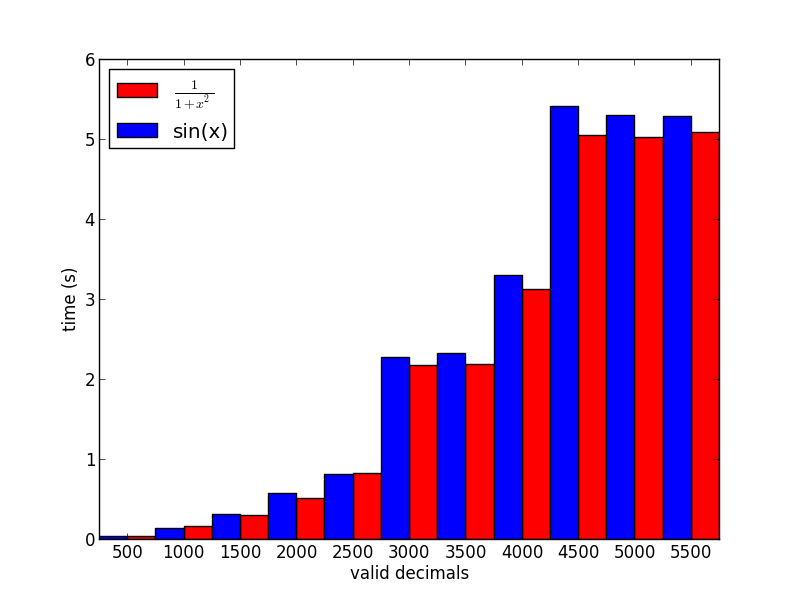
\includegraphics[width=0.5\textwidth]{img/analytic/ba_ana_dep_on_n_bar.png}
				\caption{running time evaluating \baana at fixed point $x=0.8$ depending on the desired number of valid decimals}
				\label{fig:ba_ana dep on n}
			\end{figure}
			\begin{figure}[h]
				\centering
				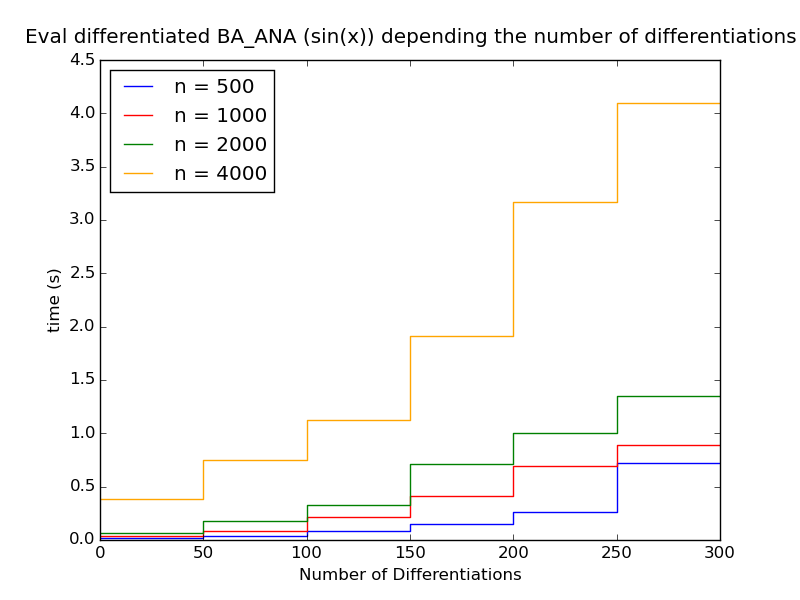
\includegraphics[width=0.5\textwidth]{img/analytic/ba_ana_dep_on_diff_sin.png}
				\caption{running time evaluating differentiated \baana with series for $\sin(x)$ at fixed point $x=0.8$ with different numver of desired valid decimals depending on the number of differentiation}
				\label{fig:ba_ana dep on differentiation}
			\end{figure}
			Running time Integration, Differentiation, Coefficient computation 
		\subsection{\anarect}
			Since most operations on the power series on \anarect and \baana are identical ‚and are therefore expected to behave similiarily, 
			the crucial part of evaluating \baana is the evaluation using analytic continuation.
			
			In particular the following questions
			\begin{enumerate}
				\item How does the running time depend on the number of analytic continuations and on the output precision?
				\item How many coefficients of each power series are needed?
				\item How does the number of coefficients needed grow with the number of iterations and the output precision?
			\end{enumerate} 

		From the theoretical analysis, the expected behavior is that the running time for evaluating at a fixed 
		point is bounded by $O(n^4)$ and should grow exponentially with the number of analytic continuations.
		The number of coefficients needed from the first series should grow similiarly. 

 		Evaluation was performed on test functions, in particular the functions $x \to sin(x)$, $x \to \frac{1}{1+x^2}$, $x \to ln(2+x)$ and $x \to \sqrt{2+x}$. 

 		Due to the iterative concept of the \irram, the running time is not continuous in the desired output precision, but grow stepwise with the internal precision of the \irram.

		\begin{figure}[h]
			\centering
			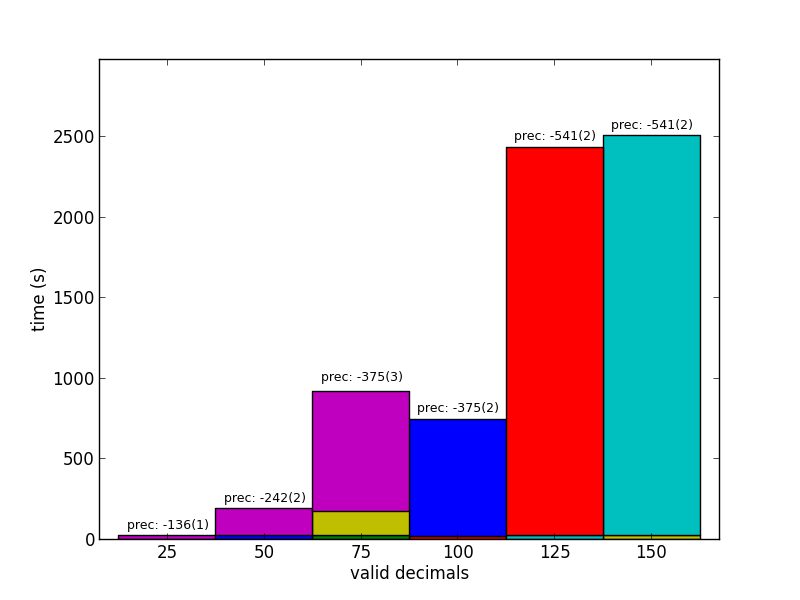
\includegraphics[width=0.5\textwidth]{img/analytic/sin_for_series_4_dep_on_n.png}
			\caption{running time of \anarect computing the sine function at the boundary of the third series, depending on the number of valid digits. The text above the bars shows the highest internal precision and the number of iterations \irram did.}
			\label{fig:sin dep on n}
		\end{figure}

		Figure \ref{fig:sin dep on n} shows, how the running time of evaluating at a fixed point $x$ depends on the desired number of valid decimals. 
		$x$ is chosen so that $3$ analytic continuations are necessary. 

		The plot also contains the information on how many iterations \irram performed and the maximum internal 
		precision (text above the bars). 
		Every bar is broken down into smaller bars, that show how much time was spent in each iteration of the \irram.
		The reason for the running time going down again between $75$ and $100$ decimals is, that
		the iterations do not always have the same size, but \irram makes estimates on a good step size.
		The internal precision in the end is $-375$ for both $n=75$ and $n=100$, but 
		for $75$ the first estimate is too small, leading to a total number of $3$ iterations instead of only $2$ iterations for $n=100$.
		However, the plot also clearly shows that the running time is always dominated by the time spent in the last iteration.

		\begin{figure}[h]
			\centering
			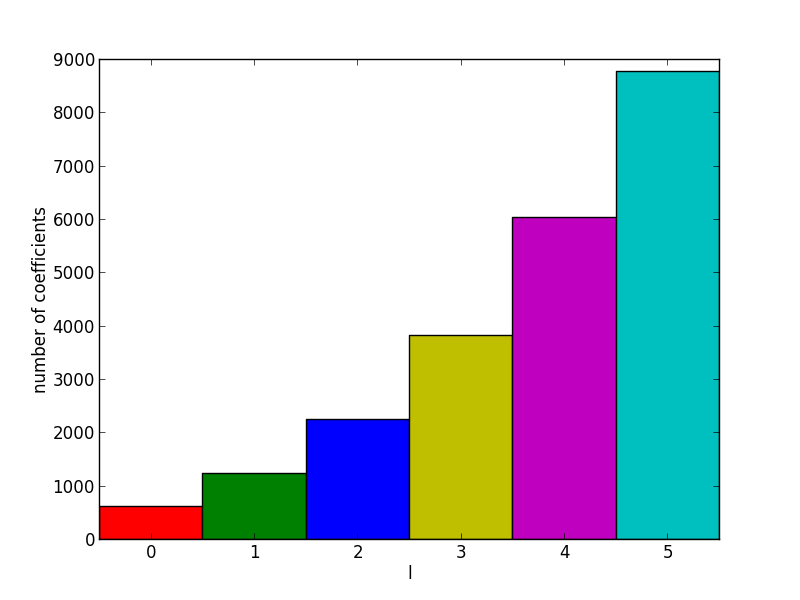
\includegraphics[width=0.5\textwidth]{img/analytic/sin_for_coeffs_prec_150_dep_on_series.png}
			\caption{Number of coefficients read from the original series when evaluating sine-function with 150 valid decimals, depending on the number of analytic continuations}
			\label{fig:sin dep on n}
		\end{figure}

		\begin{figure}[h]
			 \centering
			\begin{subfigure}{0.48\textwidth}
				\centering
			  	\begin{tabular}{|c|c|c|}
			  	\hline
			  	prec & $N^{(1)}$ & sec \\
			  	\hline
			  	50 & 71 & 0\\
			  	\hline
			  	136 & 271 & 0\\
			  	\hline
			  	242 & 527 & 2\\
			  	\hline
			  	375 & 842 & 6\\
			  	\hline
			  	541 & 1235 & 20\\
			  	\hline
			  	\end{tabular}
			  	\caption{evaluating at series 1}
		  	\end{subfigure}
			\begin{subfigure}{0.48\textwidth}
				\centering
			  	\begin{tabular}{|c|c|c|c|c|c|}
			  	\hline
			  	prec & $N^{(0)}$ & $N^{(1)}$ &$N^{(2)}$ & $N^{(3)}$ & $N^{(4)}$ \\
			  	\hline
			  	50 & 13 & 30 & 59 & 112 & 212\\
			  	\hline
			  	136 & 55 & 120 & 234 & 442 & 833\\
			  	\hline
			  	242 & 109 & 236 & 458 & 863 & 1626\\
			  	\hline
			  	375 & 175 & 378 & 733 & 1382 & 2603\\
			  	\hline
			  	541 & 258 & 556 & 1078 & 2031 & 3825\\
			  	\hline
			  	\end{tabular}
			  	\caption{evaluating at series 3}
		  	\end{subfigure}
          % \begin{tabular}{|c||c|c|c|c|c|}
          % \hline
          % prec & $N^{(0)}$ & $N^{(1)}$ &$N^{(2)}$ & $N^{(3)}$ & $N^{(4)}$ \\
          % \hline\hline
          % 50 & 12 & 31 & 63 & 121 & 229\\
          % \hline
          % 136 & 55 & 136 & 276 & 531 & 1009\\
          % \hline
          % 242 & 107 & 248 & 493 & 939 & 1778\\
          % \hline
          % 375 & 175 & 393 & 773 & 1466 & 2769\\
          % \hline
          % 541 & 258 & 571 & 1118 & 2116 & 3993\\
          % \hline
          % \end{tabular}
			\caption{Number of coefficients accessed in an iRRAM iteration of precision \sprec when evaluating at on the boundary of the first and third series.}
			\label{fig:xinv coeff 0 dep on n}
		\end{figure}

		Table \ref{fig:xinv coeff 0 dep on n} shows the number $N^{(l)}$ of coeffcients accesed from the original series, when evaluated at a point where $l$ analytic continuations are necessary depending on 
		the internal precision of \irram.

		\begin{figure}[h]
			\centering
			\begin{subfigure}{.45\textwidth}
				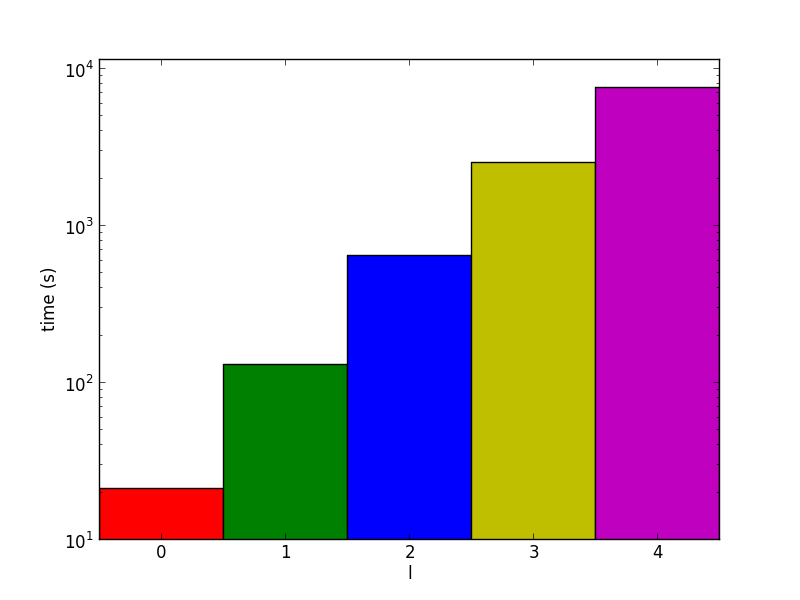
\includegraphics[width=1.0\textwidth]{img/analytic/sin_for_n_prec_150_dep_on_series_log.png}
				\caption{$x\sin(x)$}
			\end{subfigure}
			\begin{subfigure}{.45\textwidth}
				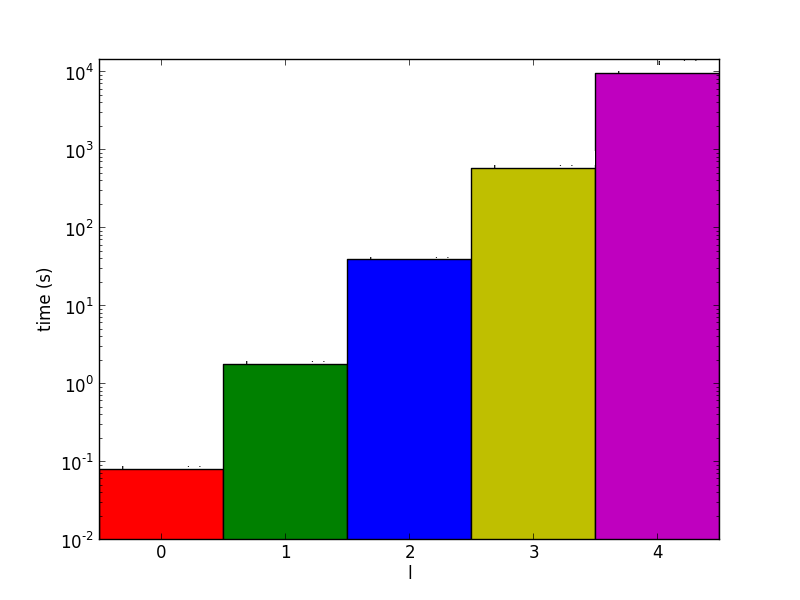
\includegraphics[width=1.0\textwidth]{img/analytic/log_for_n_prec_150_dep_on_series_log.png}
				\caption{$\log(2+x)$}
			\end{subfigure}
			\caption{log-scale plot of the running time for \anarect with 150 valid digits at the boundary of the $l$-th series.}
			\label{fig:baana dep on series}
		\end{figure}

		How the running time and the number of coefficients  depends on the number of analytic continuations can also be observed in Figure \ref{fig:baana dep on series}. 

		All in all the figures are accordance with the qualitative behaviour expected from the theoretical analysis.
	\section{Applications}